\documentclass{article}
\usepackage{listings}
\usepackage{setspace}
\usepackage{graphicx}
\usepackage{subfigure}
\usepackage{amsmath}
\usepackage{pythonhighlight}
\usepackage{longtable}
\usepackage{booktabs}
\usepackage{geometry}
\usepackage{xcolor}
\usepackage{caption}
\usepackage{amsfonts,amssymb}
\usepackage{multirow}
\usepackage{subfigure}
\geometry{a4paper,scale=0.8}
\definecolor{codegreen}{rgb}{0, 0.6, 0}
\definecolor{codegray}{rgb}{0.5, 0.5, 0.5}
\definecolor{codepurple}{HTML}{C42043}
\definecolor{backcolour}{HTML}{F2F2F2}
\lstdefinestyle{sql1}{
	language=SQL,
	frame = l,
	backgroundcolor=\color{backcolour},
	commentstyle = \color{codegreen},
	keywordstyle = \color{codepurple},
	numberstyle = \footnotesize\color{black},
	stringstyle = \color{codepurple},
	basicstyle = \footnotesize,
	breakatwhitespace = false,
	breaklines = true,
	captionpos = b,
	keepspaces = true,
	numbers = left,
	showspaces = false,
	showstringspaces = false,
	showtabs = false
}
\begin{document}
\begin{center}
	\Large DSA5104 Assignment1
\end{center}
\vspace{6 pt}
\begin{center}
	Wang Jiangyi, A0236307J
	\\
	National University of Singapore
\end{center}
%\tableofcontents

%\newpage
\section{Task 2: Schema Diagram}
\begin{figure}[h]
	\centering
	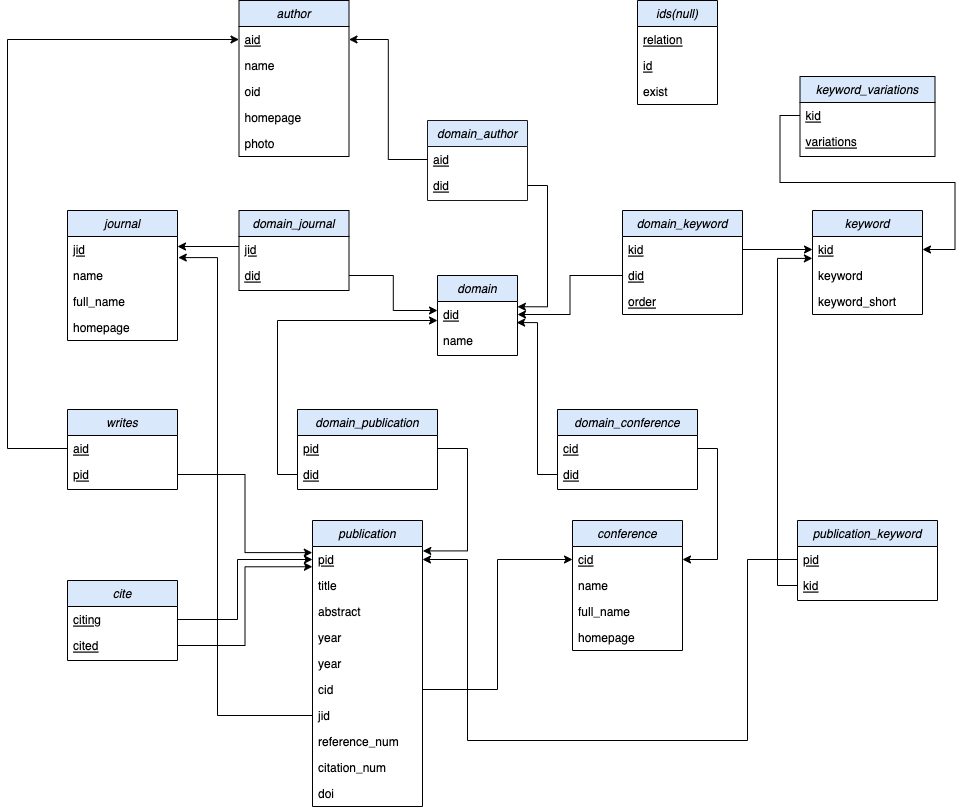
\includegraphics[width=.65\textheight]{figures/relational diagram.png}
	\caption{Relational Diagram for MAS}
	\label{fig:001}
\end{figure}
\newpage
\section{Task 3: NLQueries}
In the beginning, I pointed out that, \textbf{for Query 7 and Query 13}, I have \textbf{different understanding of NL Query}. Therefore, I give all the answers corresponding to different understanding.
\subsection{Query 1}
\textbf{NL Query:} Return me the authors who have papers in PVLDB.
\vspace{6 pt}
\\
\textbf{SQL Query: (2 methods) }
\lstinputlisting[style = sql1]{codes/q1_1320.txt}
\newpage
\textbf{Query Result: (1320 rows in total)}
\begin{figure}[h]
	\centering
	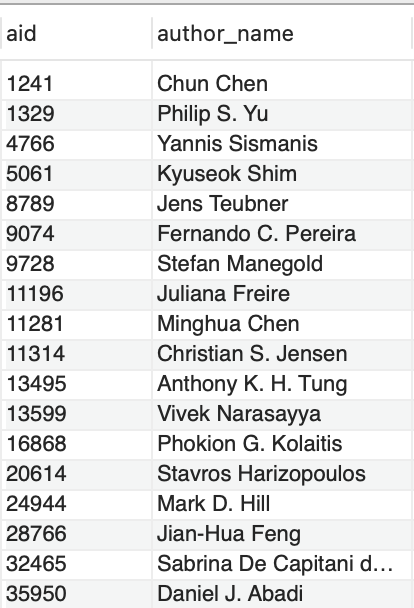
\includegraphics[width=.17\textheight]{figures/q1_res.png}
	\caption{Result for query 1}
	\label{fig:002}
\end{figure}
\subsection{Query 2}
\textbf{NL Query:} Return me the organization H. V. Jagadish is in.
\vspace{6 pt}
\\
\textbf{SQL Query: }
\lstinputlisting[style = sql1]{codes/q2_1.txt}
\textbf{Query Result: (1 row in total)}
\begin{figure}[h]
	\centering
	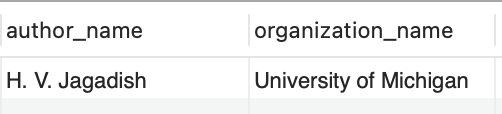
\includegraphics[width=.25\textheight]{figures/q2_res.png}
	\caption{Result for query 2}
	\label{fig:003}
\end{figure}
\subsection{Query 3}
\textbf{NL Query:} Return me the authors who have papers in VLDB conference before 2002 after 1995.
\vspace{6 pt}
\\
\textbf{SQL Query: }
\lstinputlisting[style = sql1]{codes/q3_984.txt}
\textbf{Query Result: (984 rows in total)}
\begin{figure}[h]
	\centering
	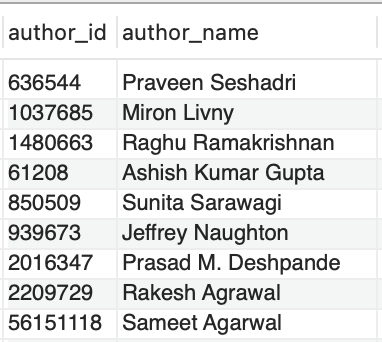
\includegraphics[width=.2\textheight]{figures/q3_res.png}
	\caption{Result for query 3}
	\label{fig:004}
\end{figure}
\subsection{Query 4}
\textbf{NL Query:} Return me the authors who have cooperated both with "H. V. Jagadish" and "Divesh Srivastava".
\vspace{6 pt}
\\
\textbf{SQL Query: }
\lstinputlisting[style = sql1]{codes/q4_48.txt}
\textbf{Query Result: (48 rows in total)}
\begin{figure}[h]
	\centering
	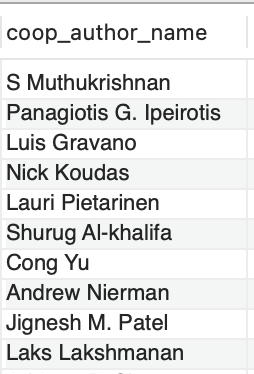
\includegraphics[width=.15\textheight]{figures/q4_res.png}
	\caption{Result for query 4}
	\label{fig:005}
\end{figure}
\subsection{Query 5}
\textbf{NL Query:} Return me the authors who have more papers on VLDB than ICDE.
\vspace{6 pt}
\\
\textbf{SQL Query:}
\lstinputlisting[style = sql1]{codes/q5_2627.txt}
\textbf{Query Result: (2627 rows in total)}
\begin{figure}[h]
	\centering
	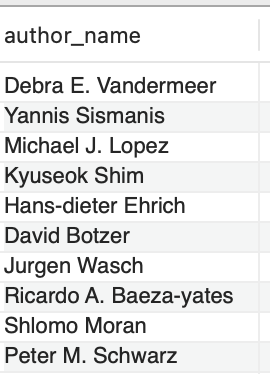
\includegraphics[width=.15\textheight]{figures/q5_res.png}
	\caption{Result for query 5}
	\label{fig:006}
\end{figure}
\subsection{Query 6}
\textbf{NL Query:} Return me the authors who have cited papers of H. V. Jagadish.
\vspace{6 pt}
\\
\textbf{SQL Query: (2 methods)}
\lstinputlisting[style = sql1]{codes/q6_7245.txt}
\textbf{Query Result: (7245 rows in total)}
\begin{figure}[h]
	\centering
	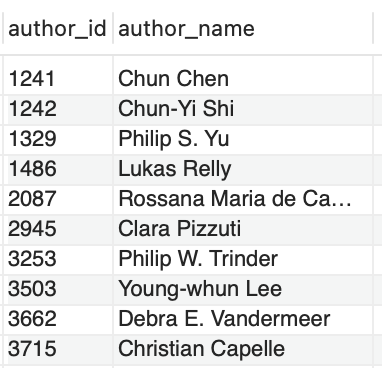
\includegraphics[width=.17\textheight]{figures/q6_res.png}
	\caption{Result for query 6}
	\label{fig:007}
\end{figure}
\subsection{Query 7}
\textbf{NL Query:} Return me all the papers, which contain the keyword "Natural Language".
\vspace{6 pt}
\\
\textit{\textbf{Note}: There are two different understanding of this NL Queriy. One is, the keyword contains "Natural Language" and the other is, the keyword is excatly "Natural Language". The 2 different SQL Queries can ben shown as follows:}
\vspace{6pt}
\\
\textbf{SQL Query 1, exactly 'Natural Language':}
\lstinputlisting[style = sql1]{codes/q7_11232.txt}
\newpage
\textbf{Query Result: (11232 rows in total)}
\begin{figure}[h]
	\centering
	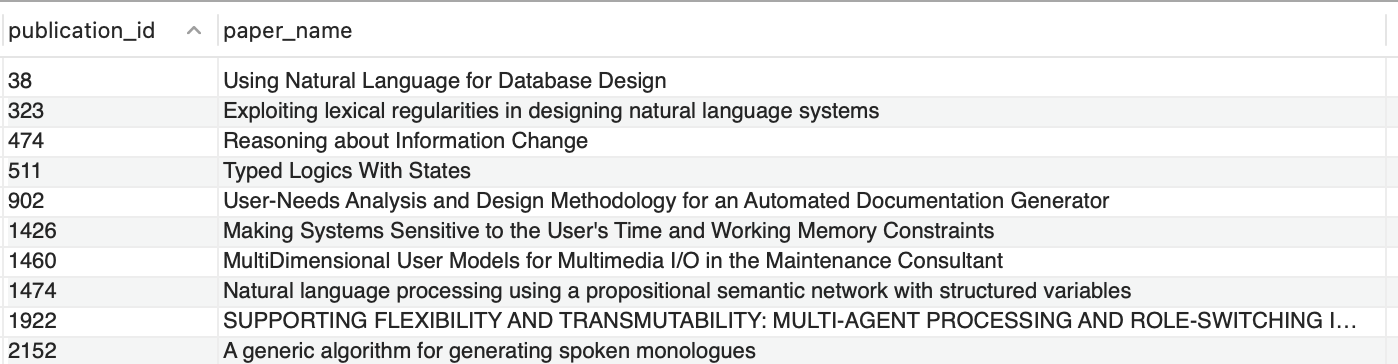
\includegraphics[width=.55\textheight]{figures/q7_res1.png}
	\caption{Result for query 7, version 1}
	\label{fig:008}
\end{figure}
\\
\textbf{SQL Query 2, contains 'Natural Language':}
\lstinputlisting[style = sql1]{codes/q7_19208.txt}
\textbf{Query Result: (19208 rows in total)}
\begin{figure}[h]
	\centering
	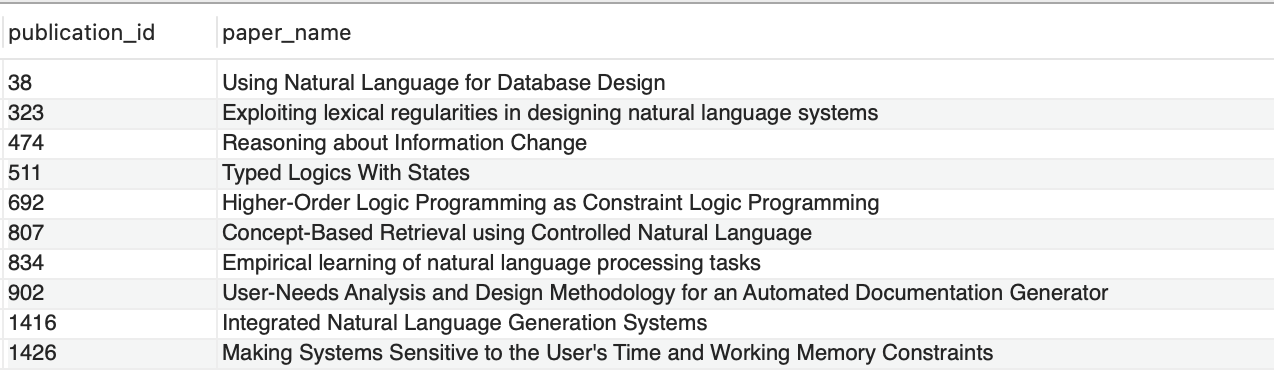
\includegraphics[width=.55\textheight]{figures/q7_res2.png}
	\caption{Result for query 7, version 2}
	\label{fig:017}
\end{figure}
\subsection{Query 8}
\textbf{NL Query:} Return me all the researchers in database area in University of Michigan.
\vspace{6 pt}
\\
\textbf{SQL Query:}
\lstinputlisting[style = sql1]{codes/q8_146.txt}
\textbf{Query Result: (146 rows in total)}
\begin{figure}[h]
	\centering
	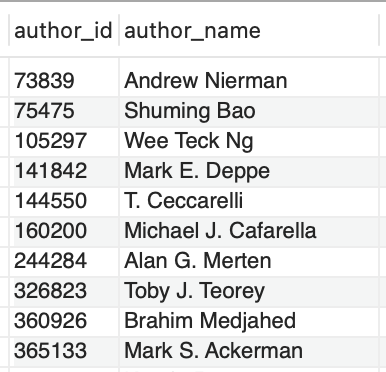
\includegraphics[width=.15\textheight]{figures/q8_res.png}
	\caption{Result for query 8}
	\label{fig:009}
\end{figure}
\subsection{Query 9}
\textbf{NL Query:} Return me the number of papers written by H. V. Jagadish, Yunyao Li, and Cong Yu.
\vspace{6 pt}
\\
\textbf{SQL Query:}
\lstinputlisting[style = sql1]{codes/q9_1.txt}
\textbf{Query Result: (1 row in total)}
\begin{figure}[h]
	\centering
	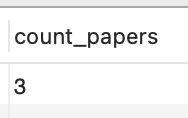
\includegraphics[width=.08\textheight]{figures/q9_res.png}
	\caption{Result for query 9}
	\label{fig:010}
\end{figure}
\subsection{Query 10}
\textbf{NL Query:} Return me the number of papers written by H. V. Jagadish in each year.
\vspace{6 pt}
\\
\textbf{SQL Query:}
\lstinputlisting[style = sql1]{codes/q10_29.txt}
\textbf{Query Result: (29 rows in total)}
\begin{figure}[h]
	\centering
	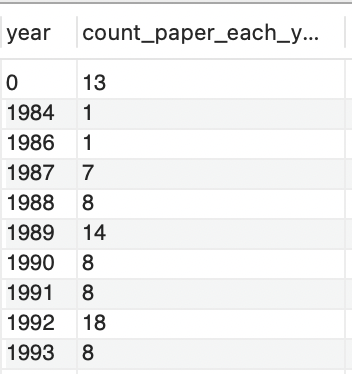
\includegraphics[width=.13\textheight]{figures/q10_res.png}
	\caption{Result for query 10}
	\label{fig:011}
\end{figure}
\subsection{Query 11}
\textbf{NL Query:}  Return me the number of citations of "Making database systems usable" in each year.
\vspace{6 pt}
\\
\textbf{SQL Query:}
\lstinputlisting[style = sql1]{codes/q11_5.txt}
\textbf{Query Result: (5 rows in total)}
\begin{figure}[h]
	\centering
	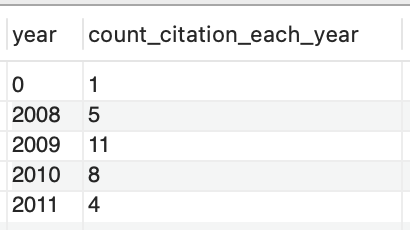
\includegraphics[width=.15\textheight]{figures/q11_res.png}
	\caption{Result for query 11}
	\label{fig:012}
\end{figure}
\subsection{Query 12}
\textbf{NL Query:}  Return me the author who has the most number of papers in the VLDB conference.
\vspace{6 pt}
\\
\textbf{SQL Query:}
\lstinputlisting[style = sql1]{codes/q12_1.txt}
\textbf{Query Result: (1 row in total)}
\begin{figure}[h]
	\centering
	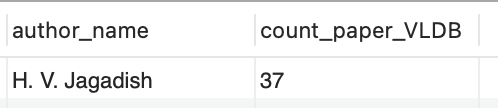
\includegraphics[width=.2\textheight]{figures/q12_res.png}
	\caption{Result for query 12}
	\label{fig:013}
\end{figure}
\subsection{Query 13}
\textbf{NL Query:}   Return me the conferences, which have more than 60 papers containing keyword "Relational Database".
\vspace{6 pt}
\\
\textit{\textbf{Note}: There are two different understanding of this NL Queriy. One is, the keyword contains "Relational Database" and the other is, the keyword is excatly "Relational Database". The 2 different SQL Queries can ben shown as follows:}
\vspace{6pt}
\\
\textbf{SQL Query 1, exactly "Relational Database":} (2 methods)
\lstinputlisting[style = sql1]{codes/q13_5.txt}
\textbf{Query Result: (5 rows in total)}
\begin{figure}[h]
	\centering
	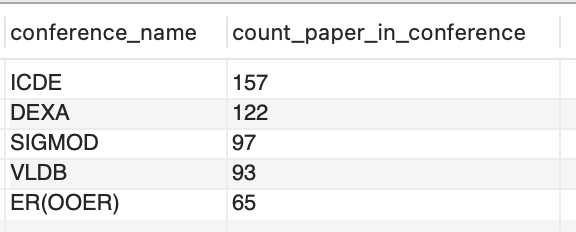
\includegraphics[width=.23\textheight]{figures/q13_res1.png}
	\caption{Result for query 13, version 1}
	\label{fig:014}
\end{figure}
\\
\textbf{SQL Query 2, contains "Relational Database":} (2 methods)
\lstinputlisting[style = sql1]{codes/q13_7.txt}
\textbf{Query Result: (7 rows in total)}
\begin{figure}[h]
	\centering
	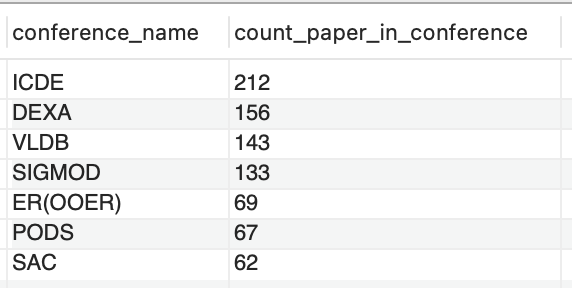
\includegraphics[width=.23\textheight]{figures/q13_res2.png}
	\caption{Result for query 13, version 2}
	\label{fig:018}
\end{figure}
\subsection{Query 14}
\textbf{NL Query:} Return me the number of papers published on PVLDB each year after 2000.
\vspace{6 pt}
\\
\textbf{SQL Query:}
\lstinputlisting[style = sql1]{codes/q14_5.txt}
\textbf{Query Result: (5 rows in total)}
\begin{figure}[h]
	\centering
	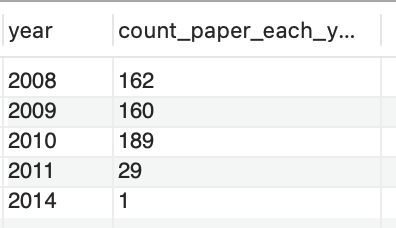
\includegraphics[width=.2\textheight]{figures/q14_res.png}
	\caption{Result for query 14}
	\label{fig:015}
\end{figure}
\subsection{Query 15}
\textbf{NL Query:} Return me the paper after 2000 in VLDB conference with the most citations.
\vspace{6 pt}
\\
\textbf{SQL Query:}
\lstinputlisting[style = sql1]{codes/q15_1.txt}
\textbf{Query Result: (1 row in total)}
\begin{figure}[h]
	\centering
	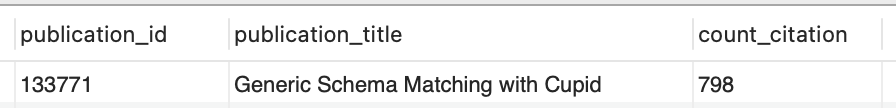
\includegraphics[width=.4\textheight]{figures/q15_res.png}
	\caption{Result for query 15}
	\label{fig:016}
\end{figure}
\end{document}